\documentclass[xcolor=pdftex,dvipsnames,table]{beamer}
 %\usecolortheme[named=OliveGreen]{structure}
 \useoutertheme{infolines}
 %\usetheme[height=7mm]{Rochester}
 \usetheme[height=7mm]{Boadilla}
\usecolortheme{seagull}
%\usecolortheme{seahorse}
%\usecolortheme{dove}

\hypersetup{colorlinks=true,linkcolor=Red}
 \setbeamertemplate{items}[ball]
 \setbeamertemplate{blocks}[rounded][shadow=true]
 \setbeamertemplate{navigation symbols}{}
\usepackage{subfigure}
\usepackage{hyperref}

\author[Group-01]{Bhavya Bhatt, GaganDeep Tomar, Shreyas Bapat}
\title[CS-671]{\textsc{Deep Learning and its Applications\\Project Presentation on MRI-Image Reconstruction\\Group-01}}
\institute[SCEE, IIT-Mandi]{
\includegraphics[scale=0.25]{logo.jpg}\\}

\date[ April 18, 2019]{April 18, 2019}
%\graphicspath{{myfigs/}}



%#make sure to change this part, since it is predefined
      %\defbeamertemplate*{footline}{infolines theme}
      \setbeamertemplate{footline}
        {
      \leavevmode%
      \hbox{%
      \begin{beamercolorbox}[wd=.333333\paperwidth,ht=2.25ex,dp=1ex,center]{author in head/foot}%
        \usebeamerfont{author in head/foot}\insertshortauthor~~(\insertshortinstitute)
      \end{beamercolorbox}%
      \begin{beamercolorbox}[wd=.333333\paperwidth,ht=2.25ex,dp=1ex,center]{title in head/foot}%
        \usebeamerfont{title in head/foot}\insertshorttitle
      \end{beamercolorbox}%
      \begin{beamercolorbox}[wd=.333333\paperwidth,ht=2.25ex,dp=1ex,right]{date in head/foot}%
        \usebeamerfont{date in head/foot}\insertshortdate{}\hspace*{2em}

    %#turning the next line into a comment, erases the frame numbers
        %\insertframenumber{} / \inserttotalframenumber\hspace*{2ex}

      \end{beamercolorbox}}%
      \vskip0pt%
    }

\begin{document}

\begin{frame}[plain]
  \titlepage
\end{frame}


\begin{frame}[plain]
   \tableofcontents
 \end{frame}
 
\section{Problem Statement}
\frame{\frametitle{Problem Statement }
A standard mri reconstruction problem can be understood with the following figure
\begin{figure}
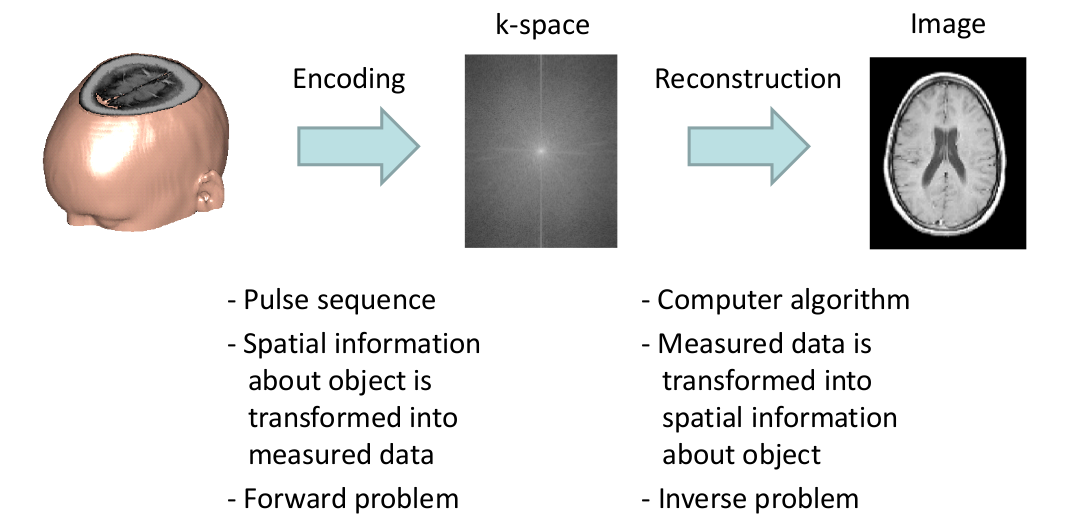
\includegraphics[width = \linewidth]{Imgs/mri_big_picture.png}
\end{figure}
}
\frame{\frametitle{Problem Statement }
\begin{enumerate}
\item k-space is fourier space and samples are collected in this space from mri machine.
\item If we had infinite points in k-space then image can be reconstructed perfectly.
\item But we only have a specific sampled portions of this k-space and so the problem is to reconstruct from these sample an image which is as close as true image.
\end{enumerate}  \vspace{10pt}
}
\section{Some Related Work}
\frame{\frametitle{Some Related Work }
The most important theorem in all of signal reconstuction field is shannon theorem which is a follows
\begin{figure}
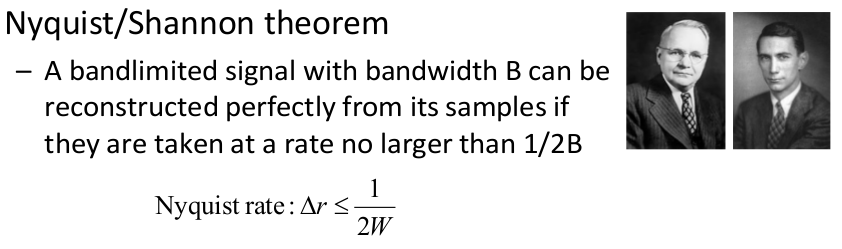
\includegraphics[width = \linewidth]{Imgs/shannon.png}
\end{figure}
\begin{enumerate}
\item This reconstruction is perfect only if we have infinte number of k-space sample points.
\item In real life scenario we only have a finite portion of these k-space samples.
\end{enumerate}
}
\frame{\frametitle{Some Related Work }
We would follow in our project sampling as follows
\begin{figure}
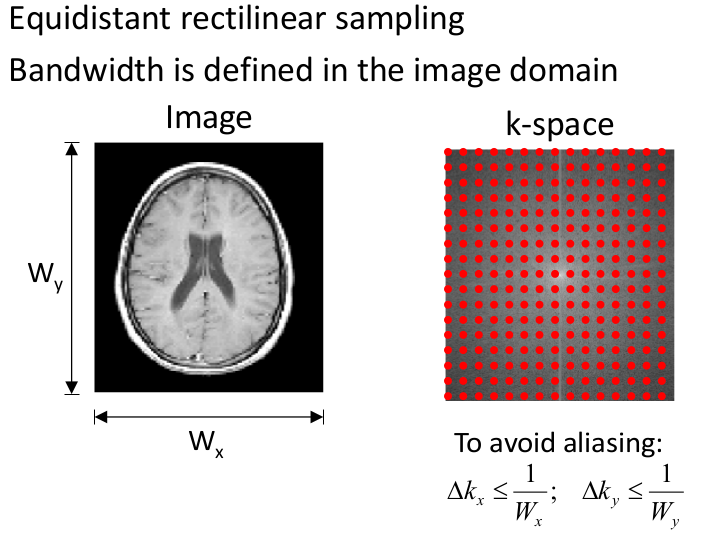
\includegraphics[width = \paperwidth]{Imgs/sampling.png}
\end{figure}
}
\section{Motivation and Challenges}
\frame{\frametitle{Motivation and Challenges }
\begin{enumerate}
\item New methods of Deep Learning can acheive state of the art performance.
\item The challenges faced while is that any architecture would involve computing fourier transforms apart from training computations and this drastically increases the training and overall model processing time.
\item This makes DL models to be very inefficient in these kinds of reconstruction problems. 
\end{enumerate}
}

\section{Dataset}
\frame{\frametitle{Dataset }
The anonymized imaging dataset provided by NYU Langone comprises raw k-space data from more than 1,500 fully sampled knee MRIs obtained on 3 and 1.5 Tesla magnets  from 10,000 clinical knee MRIs also obtained at 3 or 1.5 Tesla. Curation of these datasets are part of an IRB approved study. The raw dataset includes coronal proton density-weighted images with and without fat suppression
} 

\newpage
\section{Proposed Methodology}
\frame{\frametitle{Proposed Methodology }
The proposed flow architecture is as follows
\begin{figure}
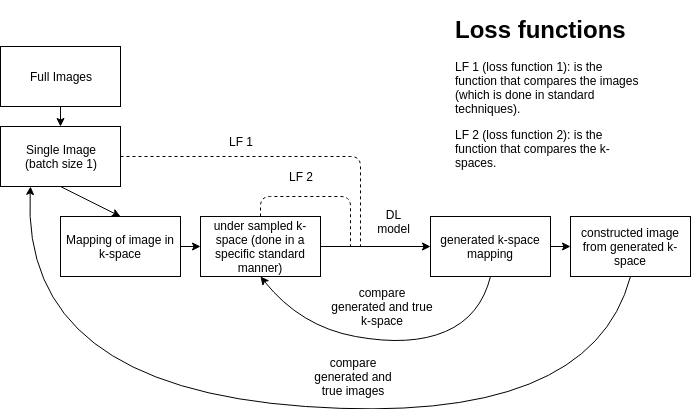
\includegraphics[width = \linewidth]{Imgs/architecture.png}
\end{figure}
}
\frame{\frametitle{Proposed Methodology }
The detailed architecture at NN level is yet to be formulated.
Some additional inputs to the above workflow can be done which are as follows
\begin{enumerate}
\item To avoid computing fourier transforms which are computationally very heavy we can instead use another network to generate these fourier transforms (as it is just a mapping).
\item To acheive a more robust model we can use a representation layer after under sampled k-space block which would learn the representation of these k-space points.
\item The representation would be such that its counter part in image space would be convolution operation.
\end{enumerate}
}

\section{Progress}
\frame{\frametitle{Progress }
\begin{enumerate}
\item Currently the code for converting images to fourier transforms is in working state.
\item Neural Network for generating the fourier transforms is in tranining phase.
\end{enumerate}
}
\section{Conclusion and Future work}
\frame{\frametitle{Conclusion and Future work}

According to the above discussion the tasks for future is 
\begin{enumerate}
\item Find good loss functions both for k-space and image space and appropiate tuning of coupling constant of the two.
\item A representation operator analogous to kernel in image space and assosiated operation analogous to convolution that can be used to represent the samples of fourier space which itself can be learnt just like  kernels are learnt in CNN.
\end{enumerate}
}






\end{document}